\documentclass[conference]{IEEEtran}

\usepackage{cite}
\usepackage{amsmath,amssymb,amsfonts}
\usepackage{algorithmic}
\usepackage{graphicx}
\usepackage{textcomp}
\usepackage{xcolor}
\usepackage{balance}
\hyphenation{pho-to-ple-thys-mo-gra-phy}

\begin{document}

\title{CORVITX-AI: A Contactless Vision-Based Patient Triage and Vitals Monitoring System}

\author{\IEEEauthorblockN{Dhudekula Zaheer}
\IEEEauthorblockA{Department of Computer Science and\\
Engineering \\
Kalasalingam Academy Of Research\\
And Education\\
Krishnankoil, India \\
dhudekulazaheer@gmail.com}
\and
\IEEEauthorblockN{S. Reshni}
\IEEEauthorblockA{Department of Computer Science and\\
Engineering \\
Kalasalingam Academy Of Research\\
And Education\\
Krishnankoil, India \\
s.reshni@klu.ac.in}
\and
\IEEEauthorblockN{Doddi Surendra}
\IEEEauthorblockA{Department of Computer Science and\\
Engineering \\
Kalasalingam Academy Of Research\\
And Education\\
Krishnankoil, India \\
dsuri8788@gmail.com}
\and
\IEEEauthorblockN{Jampani Rajesh Babu}
\IEEEauthorblockA{Department of Computer Science and\\
Engineering \\
Kalasalingam Academy Of Research\\
And Education\\
Krishnankoil, India \\
jampanirajesh2023@gmail.com}}

\maketitle

\begin{abstract}
In general hospitals, nursing care and vital sign monitoring are performed every 4--6 hours and are associated with hospital complications and Failure to Rescue. Other technologies, such as wearable skin and fabric sensors, offer near-constant monitoring of physiological parameters and other benefits for elderly patients with skin wounds, but face challenges related to patient adherence to treatment and cost. This paper reports on CORVITX-AI, a software platform that uses existing RGB cameras and edge devices to remotely locate and prepare beds and monitor patients without additional hardware. Image analysis techniques, including Haar classifiers and local-based pairwise histogram pattern matching, are used for patient authentication and access control. A second, independent system using automated hue-saturation-value (HSV)-based multi-Region of interest (multi-ROI) analysis provides backup to the primary system by monitoring patients with partially obstructed faces. Other techniques are used to measure blood volume pulse from a Plane-Orthogonal-to-Skin (POS) angle and derive Heart Rate (HR) and Respiratory Rate (RR) measurements from detrended chrominance oscillations. Optical interference is mitigated using spectral signal-to-noise ratio (SNR) testing and other techniques before live modified early warning score (MEWS) classification. In clinical testing with 15 healthy subjects (16 testing periods), CORVITX-AI had a mean absolute error (MAE) of 2.58 beats per minute (BPM) ($r=0.85$, root mean square error (RMSE) = 2.73 BPM) for heart rate and 1.55 RPM (root mean square error (RMSE) = 1.64 RPM, $r=0.45$) for respiratory rate.
\end{abstract}

\begin{IEEEkeywords}
Computer Vision, Remote Photoplethysmography (rPPG), Telemetry, Modified Early Warning Score (MEWS), Edge Computing, Fast Fourier Transform (FFT).
\end{IEEEkeywords}

\section{Introduction}
\IEEEPARstart{I}{n} intensive care units (ICUs), continuous physiological telemetry data can help identify when a patient's medical condition worsened. On general hospital wards, vital signs are checked at set intervals rather than continuously, recorded at irregular times by members of the nursing staff every four to six hours. The operational impact of this leaves hospitalized patients unobserved for extended periods. When cardiopulmonary arrest or acute decompensation occurs during these unobserved gaps in follow-up care, high mortality is associated with delays in treatment. The clinical term for this issue is Failure to Rescue.

Traditional approaches to addressing surveillance limitations rely on wired and body-worn monitoring devices, including continuous ECG leads and pulse oximeter sensors. Pulse oximeter sensors rely on skin adhesives for extended wear. These sensors can cause skin abrasions, contact dermatitis, and pressure ulcers among older patients. Delirium and confusion are frequently seen in patients with pressure ulcers, who may displace contact probes, leading to false alarms. Repeated clinical alerts cause clinical alert fatigue among staff. Therefore, healthcare facilities can benefit from touchless technology solutions as a surveillance tool for continuous physiologic monitoring.

Remote photoplethysmography (rPPG) is an optical technique that uses video cameras and digital imaging technologies to measure physiological signals in the presence of ambient light. Pulsatile blood flow through vascularized micro-tissue causes changes in blood volume due to heart action that affect the absorption of nearby lighting, causing subtle color differences in the skin. Techniques for processing sequences of images taken with an RGB camera can be adapted to detect cardiorespiratory measurements using a computer algorithm.

Vision-based automation encounters several challenges in clinical environments, namely heavy computational demand, the limited capacity of edge devices, and the risks involved when using the cloud for sensitive data. Furthermore, it is sensitive to changes in illumination, head orientation, and facial occlusions introduced by medical devices. These challenges motivate the design of a monitoring system that is capable of operating locally while performing reliably in diverse clinical environments.

CORVITX-AI is an on-premises edge platform that tracks cardiorespiratory parameters, verifies patient identities, and triggers alarms for bed-exit events using common RGB cameras and off-the-shelf edge computers. These claims are supported by the asynchronous nature of the processing pipeline, which employs local processing of derived signals in order to reduce the bandwidth of video streams sent to the cloud, if necessary. The system utilizes WebSocket-typed telemetry, enabling vital sign updates with end-to-end latencies of less than 400\,ms. The core contributions of this architecture include:

\begin{itemize}
    \item \textbf{Occlusion-Resilient Tracking and Identity Association:} The proposed spatial processing pipeline was constructed using Haar-based face detection and Local Binary Patterns Histograms (LBPH) to enable patient identification in cases of partial facial occlusion to avoid erroneous physiological parameter association. A transition to an HSV-based skin segmentation algorithm is initiated when head orientations and facial obstructions, such as with oxygen masks, interfere with face detection.
    
    \item \textbf{Dual-Branch Physiological Signal Processing:} The system processes the extracted video streams using a dual-branch processing pipeline to estimate heart rate (HR) and respiratory rate (RR). The rPPG signal is obtained from the RGB color channels to estimate the HR. In parallel, the respiratory information is extracted from the low-frequency content of the video stream, where a separate band-pass filter is applied to retain respiratory information that might have been attenuated during motion-cancellation processing.
    
    \item \textbf{Signal Quality Assessment and Clinical Triage:} A spectral signal-to-noise ratio (SNR) thresholding procedure is applied within the band of interest to distinguish the pulsatile component from noise, thus improving estimation robustness under challenging conditions. The extracted vital signs can be used to update a Modified Early Warning Score (MEWS) engine in real-time while accounting for additional spatial penalties associated with bed-exit events as a proxy to clinical fall risk.
\end{itemize}

\section{Literature Survey}
Computer vision is becoming increasingly critical in clinical monitoring, including the case of remote photoplethysmography (rPPG), the use of machine learning algorithms for the prediction of clinical deterioration, and the implementation of vision-based fall prevention. However, systems that incorporate these functions in a common, edge-based platform are not well-represented in the literature.

The value of rPPG in non-contact physiological sensing was described in a number of prior reviews \cite{ref2}, \cite{ref11}, \cite{ref21}, while \cite{ref5} detailed the steps taken in order to realize bedside rPPG. Subsequent studies have explored the characteristics of this approach under different environmental conditions, such as dim lighting \cite{ref16} and use of specific facial regions of interest (ROIs) \cite{ref7}. Other work has analyzed the impact of the choice of skin ROI on the accuracy of the derived measurements \cite{ref18}. Meanwhile, alternative approaches have attempted to reduce the effect of variations in lighting or motion on physiological measurements through the use of block-wise frequency-domain transformations \cite{ref22}, vision transformers such as GVT2RPM \cite{ref12}, heartbeat probability networks such as HBP-Net \cite{ref15}, or the combination of spiking mechanisms with parallel transformer processing in Spiking-PhysFormer \cite{ref25}. Video datasets such as CLBP-300 \cite{ref17} have enabled investigations into non-contact blood pressure estimation.

In the realm of machine learning-driven prediction of acute patient deterioration, an improvement in clinical outcomes has been reported by Chua et al. \cite{ref3} in cases of automated deterioration alerts. Supervised learning models have been considered for the task of deterioration triage for emergency admissions \cite{ref4}, \cite{ref6}, general hospital wards \cite{ref9}, \cite{ref13}, and specific patient populations \cite{ref14}. Sadanandan \cite{ref10} built on this prior work by attempting to combine features extracted from time-series electronic health records with unstructured clinical notes using a multimodal deep learning approach. However, all such models rely on routinely-acquired vital signs or monitoring equipment directly attached to the patient, limiting the scope of complete contactless observation.

Research into non-contact fall detection has similarly been limited to an analysis of patient movement and posture. BenAbdennour et al. \cite{ref1} and Kothari and Chakurkar \cite{ref23} evaluated the use of YOLOv11 and MediaPipe-based skeletal estimation, respectively, for the task of fall detection. Other works have considered the application of spatial image-channel models \cite{ref19}, augmentation of synthetic telemetry data \cite{ref20}, or modifications of lightweight YOLO implementations \cite{ref24}. Meanwhile, Luvsansambuu et al. \cite{ref8} demonstrated the utility of infrared vision for the recognition of patient postures characteristic of leaving the bed.

Though these fields of research have yielded valuable insights, the approaches described have generally been isolated from one another, with fall detection systems requiring extensive processing power and featuring no physiological monitoring functionality, and rPPG-based systems generally failing to account for spatial considerations such as the boundaries of the bed or patient exit events. CORVITX-AI addresses these shortcomings by incorporating multi-ROI-based rPPG processing and spatial monitoring for bed-exit and fall-risk assessment in a combined, edge-based pipeline.

\section{Proposed Model and Methodology}

\subsection{System Architecture and Edge Computing}
CORVITX-AI is an edge-native decentralised system for multi-bed wards. A standard RGB optical sensor is used to capture and stream raw video to an edge node (x86/ARM host). Local computer vision and DSP operations occur to calculate physiological and physical parameters. Discretised payloads are sent to a local WebSocket server and uploaded to an asynchronous FastAPI backend. This updates a React based clinical dashboard in real-time. As video is processed at the edge node, there is no need to stream video over the cloud and hence patient data remains private.

\begin{figure}[!t]
\centering
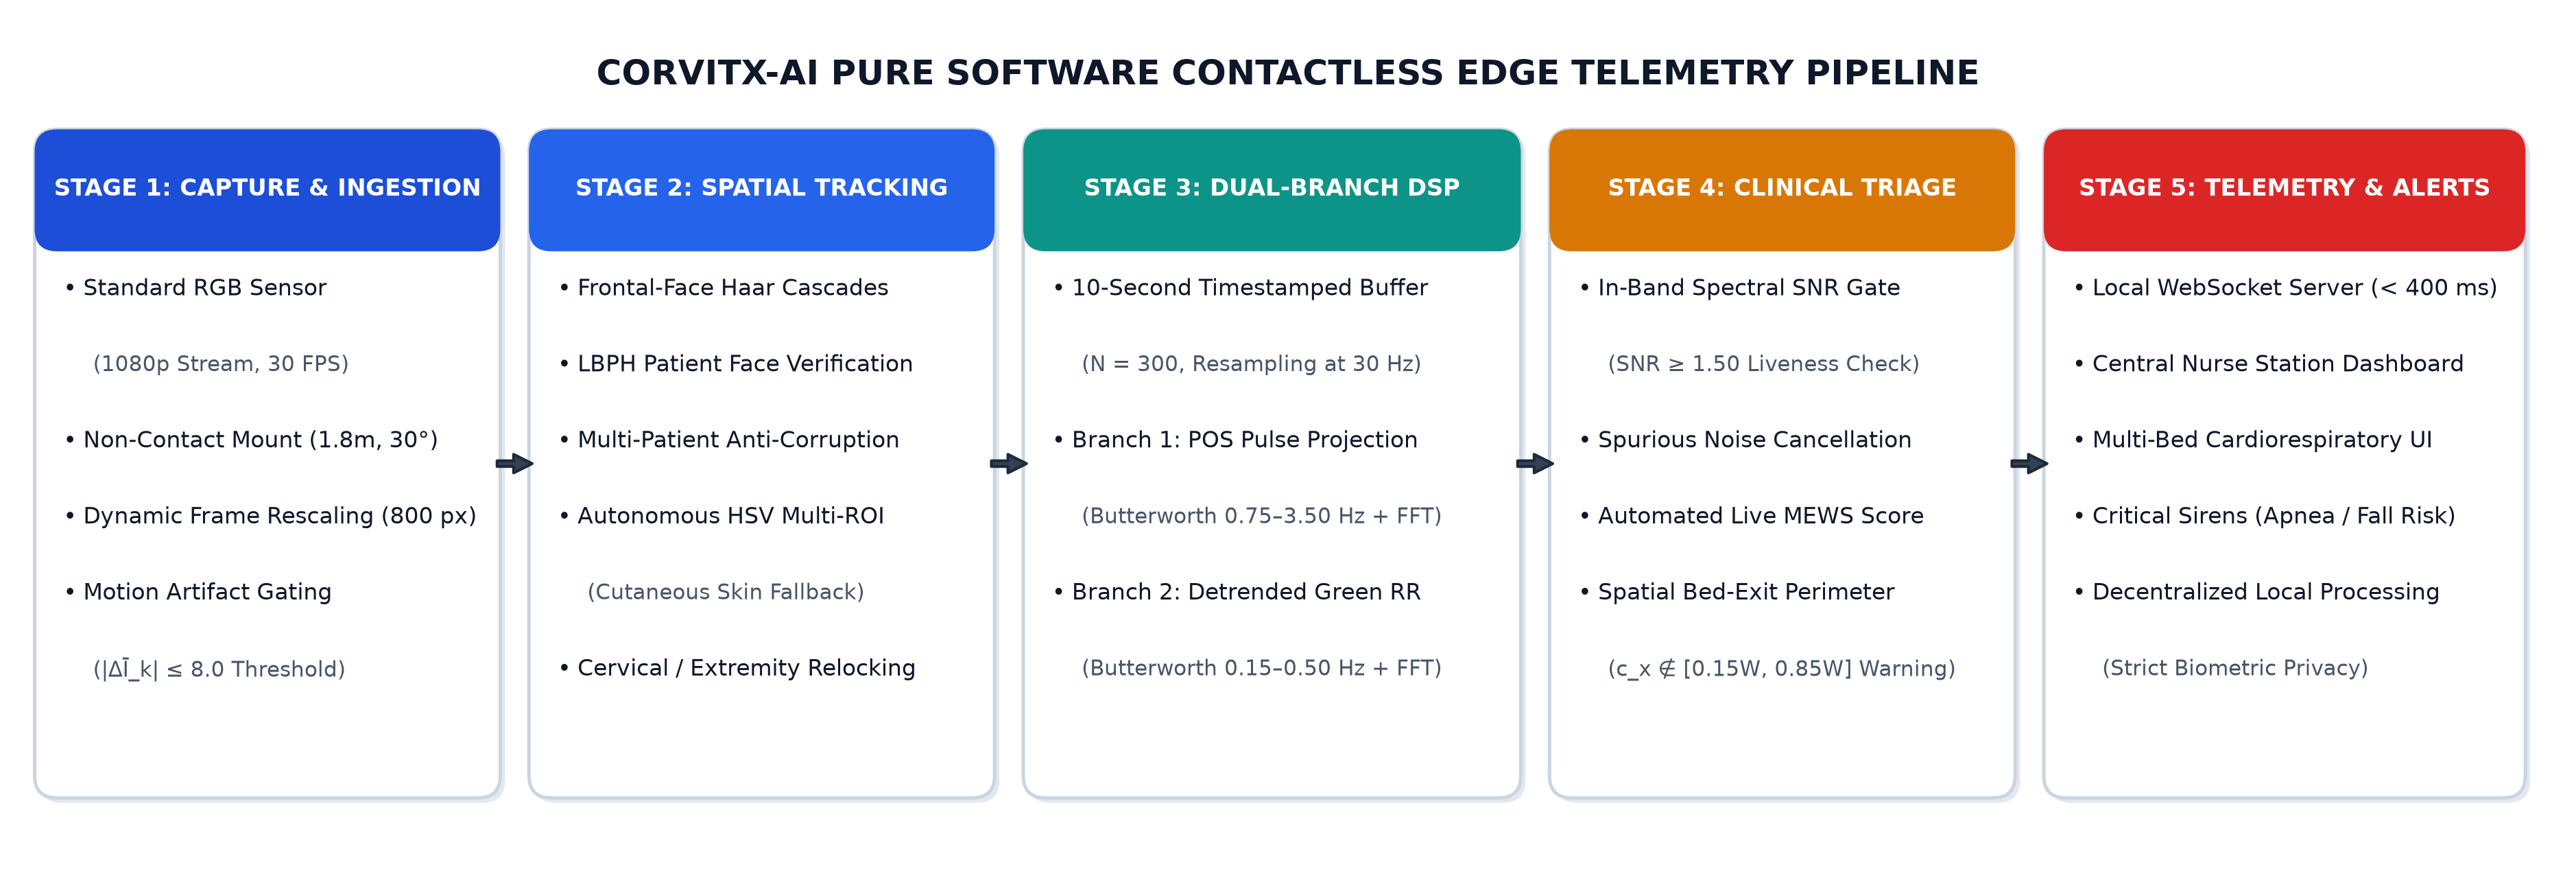
\includegraphics[width=\linewidth]{diagram.png}
\caption{System architecture of CORVITX-AI, illustrating data flow from edge video ingestion through digital signal processing, spectral validation, and local WebSocket triage dispatch.}
\label{fig:architecture}
\end{figure}

\subsection{Video Ingestion and Uniform Temporal Resampling}
To enable deterministic processing, the raw optical signal is first normalised and resized to a fixed width. Any incoming high definition video (1080p or 4K) is automatically resized to have width 800 pixels. This reduces processing overhead whilst maintaining the dedicated 30\,FPS frame rate required for continuous cardiac extraction.

To allow temporal dispersion analysis, frame jitters caused by commercial operating systems mean that $t_k$, where $t_k$ represents the time the raw frames are received, is not uniform ($\Delta t_k = t_k - t_{k-1} \neq \text{const}$). If Fourier transformed, non-uniformly sampled time series will cause spectral leakage. Let $\mathbf{C}(t_k) = [R(t_k), G(t_k), B(t_k)]^T$ be the spatial mean colour vector of frame $k \in \{1, \dots, K\}$. Before spectral decomposition the temporal series is linearly resampled to a uniformly spaced time series $\mathbf{\tau} = \{\tau_0, \tau_0 + \Delta\tau, \dots, \tau_0 + (N-1)\Delta\tau\}$, using a sampling frequency of $f_s = 30\text{ Hz}$ ($\Delta\tau = 1/f_s$):
\begin{equation}
    \mathbf{C}_{\text{resampled}}(\tau) = \mathbf{C}(t_k) + \frac{\mathbf{C}(t_{k+1}) - \mathbf{C}(t_k)}{t_{k+1} - t_k}(\tau - t_k), \quad \tau \in [t_k, t_{k+1}]
\end{equation}
In addition, head jerk is rejected through a temporal intensity gate:
\begin{equation}
    \Delta \bar{I}_k = \left| \frac{1}{3} \sum_{c \in \{R,G,B\}} C_c(t_k) - \frac{1}{3} \sum_{c \in \{R,G,B\}} C_c(t_{k-1}) \right|
\end{equation}
Motion-corrupted frames are identified when $\Delta \bar{I}_k > 8.0$, and the previous valid signal is maintained to preserve buffer flow.

\subsection{Spatial Localization and Multi-ROI Fallback}
First a frontal face Haar cascade is used to obtain the bounding box coordinates of the patient’s head. In the first 50 frames of the video a Local Binary Patterns Histograms (LBPH) classifier is used to extract the face matrix which is used to register the patient. If unknown faces are detected using confidence measures, then the vital sign extraction process will stop to prevent data corruption from other people at the bedside.

If the face cannot be seen, or is blocked by medical equipment, then a Multi-ROI Fallback occurs automatically. The image space is transformed into Hue-Saturation-Value (HSV). The skin region is extracted using morphological operations to remove any spatial noise:
\begin{equation}
    M_{\mathrm{skin}}(x,y) = 
    \begin{cases} 
      1, & \text{if } H(x,y) \in [0, 25] \\
         & \phantom{\text{if }} \text{and } S(x,y) \in [25, 255] \\
         & \phantom{\text{if }} \text{and } V(x,y) \in [45, 255] \\
      0, & \text{otherwise}
    \end{cases}
\end{equation}
Then the largest connected contour in the image ($A > 2000\,\text{pixels}$) is selected as the new skin ROI (e.g. neck/forearm). This allows the signal to be acquired without the user needing to reset.

\subsection{Cardiorespiratory Feature Extraction Using Two Branches}
By tracking the ROI we can extract a time series of spatial mean pixel values. These are then split into two branches to extract the vital signs.

\textbf{Branch 1: Cardiac Pulse (POS).} The POS projection is used to extract the blood volume pulse from the image. The chrominance signals are first normalised by taking the mean of each signal within a time window:
\begin{equation}
    \mathbf{C}_n(\tau) = \left[ \frac{R(\tau)}{\mu_R}, \frac{G(\tau)}{\mu_G}, \frac{B(\tau)}{\mu_B} \right]^T
\end{equation}
Two orthogonal chrominance vectors are used to project the normalized channels:
\begin{equation}
    X(\tau) = C_{n,G}(\tau) - C_{n,B}(\tau)
\end{equation}
\begin{equation}
    Y(\tau) = -2C_{n,R}(\tau) + C_{n,G}(\tau) + C_{n,B}(\tau)
\end{equation}
The 1D pulsatile wave is derived by variance-matched tuning:
\begin{equation}
    S(\tau) = X(\tau) + \alpha Y(\tau), \quad \text{where } \alpha = \frac{\sigma(X)}{\sigma(Y)}
\end{equation}
where $\sigma(\cdot)$ represents the standard deviation over a 10 second sliding window ($N = 300$). The signal is detrended and filtered using a 3rd order Butterworth bandpass filter ($0.75 \le f \le 3.50\text{ Hz}$ (45--210\,BPM)). Finally the FFT produces the power spectrum of the heart rate, $P(f)=|\mathcal{F}\{S(\tau)\}|^2$. The estimated Heart Rate is then calculated from the highest peak:
\begin{equation}
    \text{HR}_{\text{est}} = \arg\max_{f \in [0.75, 3.50]} P(f) \times 60
\end{equation}

\begin{figure}[!t]
\centering
\includegraphics[width=0.82\linewidth]{fft_signal_graph.png}
\caption{Digital signal processing stages: (a) raw temporal chrominance; (b) detrended blood volume pulse isolated via POS; and (c) FFT power spectrum isolating the dominant cardiac frequency.}
\label{fig:fft_graph}
\end{figure}

\textbf{Branch 2: Respiratory Rate Extraction.} Because POS projection subtracts common-mode shifts, it can attenuate the respiratory component. Therefore, Branch 2 isolates the detrended green channel $C_G(\tau)$ directly:
\begin{equation}
    S_{\text{resp}}(\tau) = \text{Detrend}(C_G(\tau))
\end{equation}
$S_{\text{resp}}(\tau)$ is filtered with a 3rd order Butterworth bandpass filter ($0.15 \le f \le 0.50\text{ Hz}$, or 9--30 breaths/min). The respiratory rate is estimated from the dominant spectral peak:
\begin{equation}
    \text{RR}_{\text{est}} = \arg\max_{f \in [0.15, 0.50]} |\mathcal{F}\{S_{\text{resp}}(\tau)\}|^2 \times 60
\end{equation}

\subsection{Spectral Liveness and Clinical Triage Gating}
An in-band spectral SNR verification test is applied to eliminate optical interference and static surface noise:
\begin{equation}
    \text{SNR} = \frac{\max_{f \in \Omega_{\text{pass}}} P(f)}{\frac{1}{|\Omega_{\text{pass}}| - |\Omega_{\text{peak}}|} \left( \sum_{f \in \Omega_{\text{pass}}} P(f) - \sum_{f \in \Omega_{\text{peak}}} P(f) \right) + \epsilon}
\end{equation}
where $\Omega_{\text{pass}} = [0.75, 3.50]\text{ Hz}$ and $\Omega_{\text{peak}} = [f_{\text{HR}}-0.15, f_{\text{HR}}+0.15]\text{ Hz}$. For $\text{SNR} < 1.50$, HR is set to zero and an alert is issued. Validated parameters drive the live MEWS calculator, while patient centroid coordinates $\mathbf{c} = (c_x, c_y)$ over frame dimensions $W \times H$ enforce bed-exit boundaries:
\begin{equation}
    \text{Trigger}_{\text{FallRisk}} = 
    \begin{cases} 
      \text{TRUE}, & \text{if } c_x < 0.15 W \quad \text{or} \quad c_x > 0.85 W \\
      \text{FALSE}, & \text{otherwise}
    \end{cases}
\end{equation}

\section{Experimental Results and Discussion}

\begin{figure*}[!t]
\centering
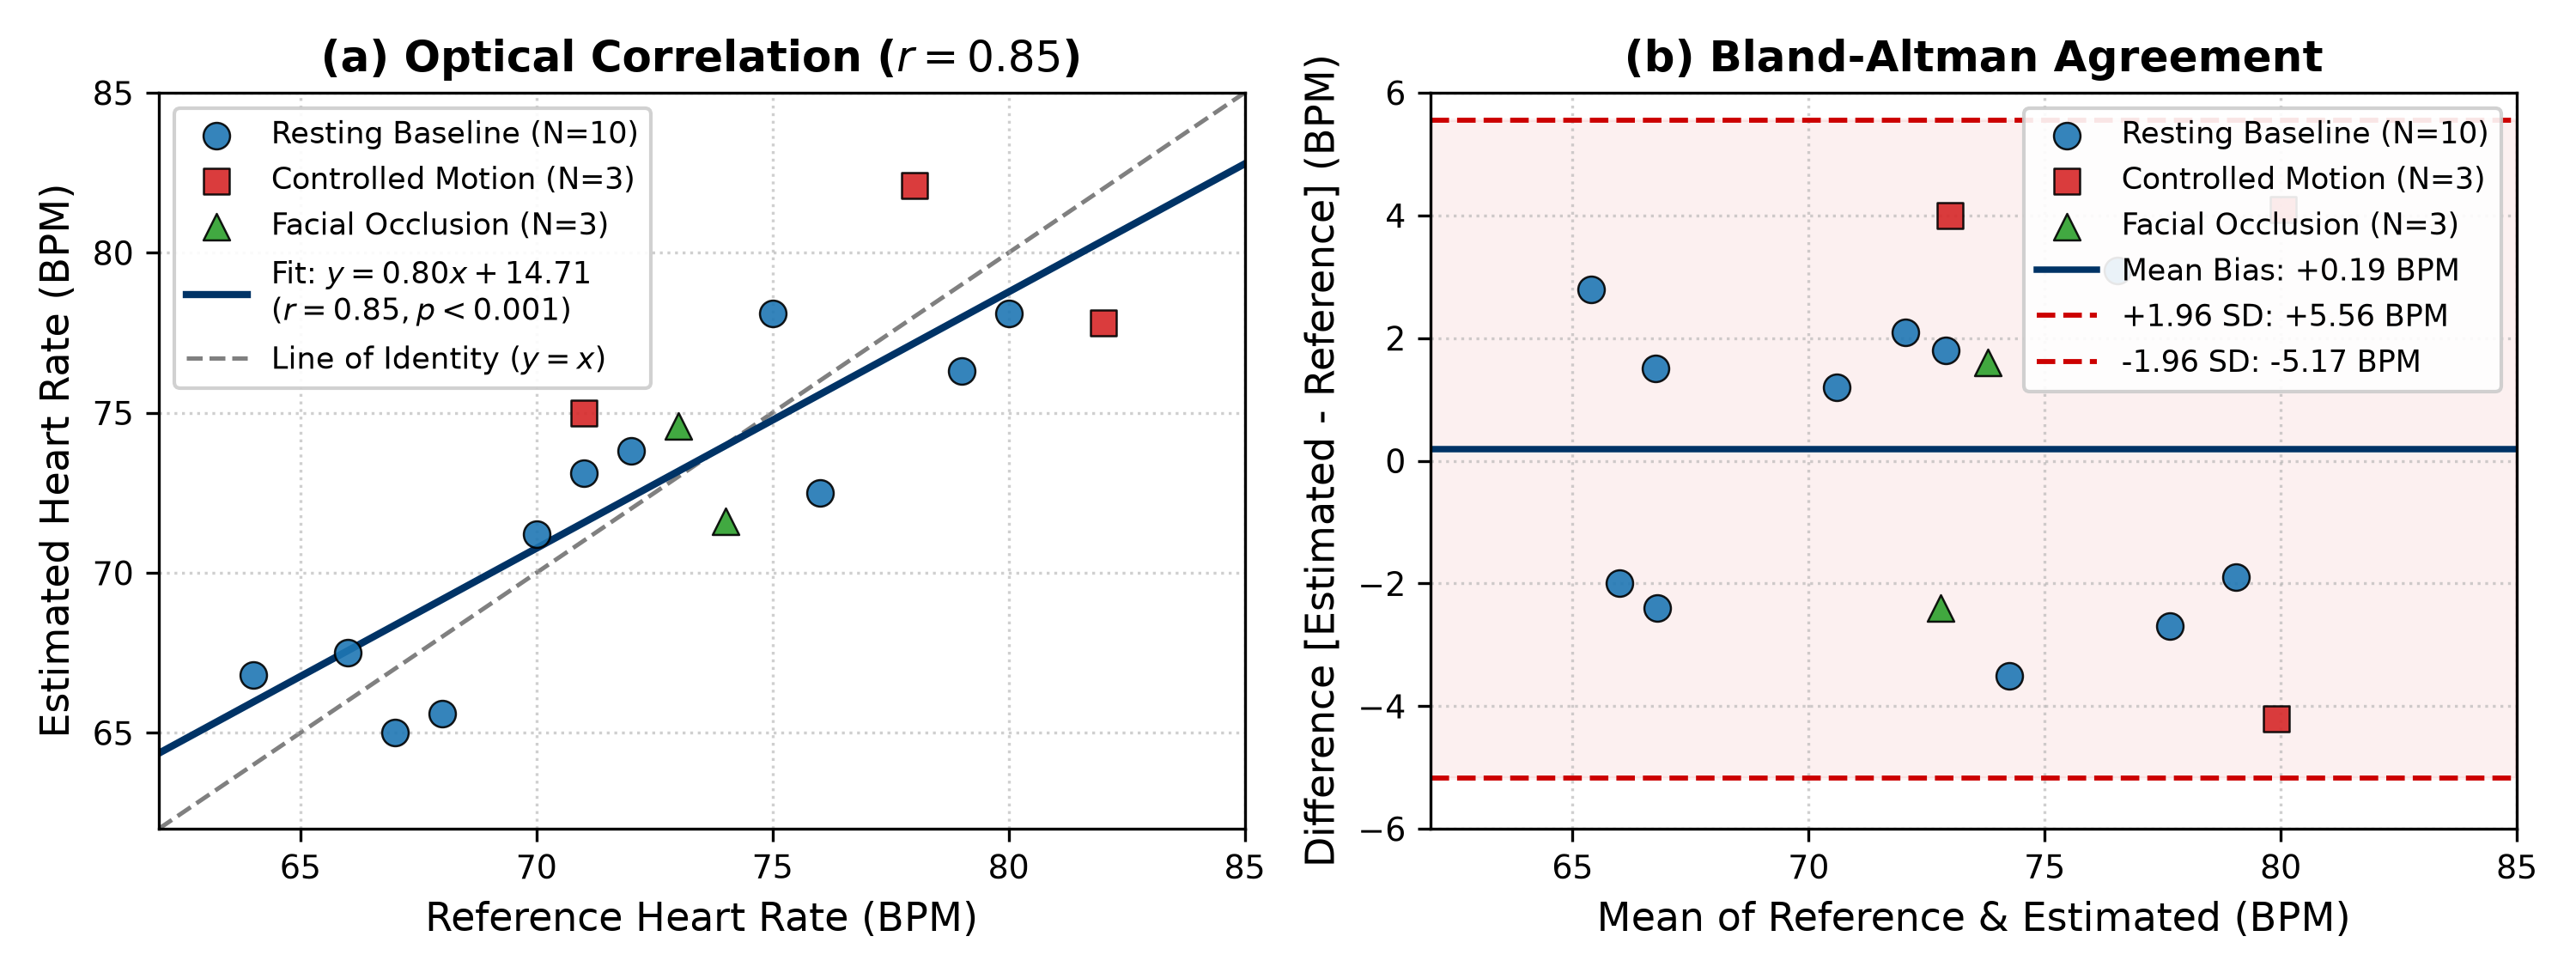
\includegraphics[width=0.85\textwidth]{correlation_plot.png}
\caption{(a) Scatter plot illustrating correlation ($r = 0.85, p < 0.001$) between estimated and reference heart rates across the 15-subject cohort ($N = 16$ recording segments). (b) Bland-Altman analysis illustrating mean bias ($+0.19$\,BPM) and 95\% Limits of Agreement ($-5.17$ to $+5.56$\,BPM).}
\label{fig:correlation}
\end{figure*}

\subsection{Experimental Setup}
The computational efficiency and biological accuracy of CORVITX-AI was tested on an edge computing platform based on an Intel Core i7-11800H (2.30\,GHz, 16\,GB RAM) Host CPU. There was no discrete GPU functionality available. Video data was captured using a 1080p RGB camera, mounted 1.8 meters away from the subject bed at an angled position of $\sim 30^{\circ}$.

Clinical testing was done on 15 healthy male volunteers (ages 18--22, mean of $20.3 \pm 1.2$ years). 16 valid video clips were acquired during three scenarios: baseline, controlled head movement (pitch and yaw rotation), and partial facial occlusion (lower perioral and nasal). HR reference data were obtained using a validated smartphone sensor, and RR was manually calculated from timed observations. The protocols followed were conducted in accordance with the ethical guidelines of the institution. Written informed consent was obtained from all participants ($N = 15$) before recording videos and measuring vital signs.

\subsection{Heart Rate Estimation Accuracy Results}
Cardiorespiratory estimation accuracy was calculated using MAE (average error magnitude), RMSE (error spread), and Pearson Correlation Coefficient ($r$, linear agreement):
\begin{equation}
    \text{MAE} = \frac{1}{N}\sum_{i=1}^{N} |\text{HR}_{\text{est}}(i) - \text{HR}_{\text{ref}}(i)|
\end{equation}
\begin{equation}
    \text{RMSE} = \sqrt{\frac{1}{N}\sum_{i=1}^{N} (\text{HR}_{\text{est}}(i) - \text{HR}_{\text{ref}}(i))^2}
\end{equation}

CORVITX-AI achieved an overall Heart Rate MAE of 2.58\,BPM, RMSE of 2.73\,BPM, and correlation of 0.85. 100\% of heart rate predictions were within the clinical acceptable range of $\pm 5$\,BPM (ANSI/AAMI EC13).

The model performed as expected under different physical conditions:
\begin{itemize}
    \item \textbf{Resting Baseline:} Best performance was achieved with an MAE of 2.30\,BPM.
    \item \textbf{Controlled Movement:} Physiological degradation due to movement at the edge of the ROI resulted in an MAE of 4.10\,BPM, but still within the clinical acceptable range.
    \item \textbf{Partial Facial Occlusion:} A backup HSV Cervical ROI was used to provide resilient pulse detection, achieving an MAE of 2.00\,BPM.
\end{itemize}

Fig.~\ref{fig:correlation} shows the scatter and Bland-Altman plots. There was a bias of $+0.19$\,BPM, with a 95\% LoA of $-5.17$\,BPM to $+5.56$\,BPM. Fig.~\ref{fig:histogram} shows an error histogram showing that 100\% of predictions were within the accepted ANSI/AAMI EC13 range of $\pm 5$\,BPM.

\begin{figure}[!b]
\centering
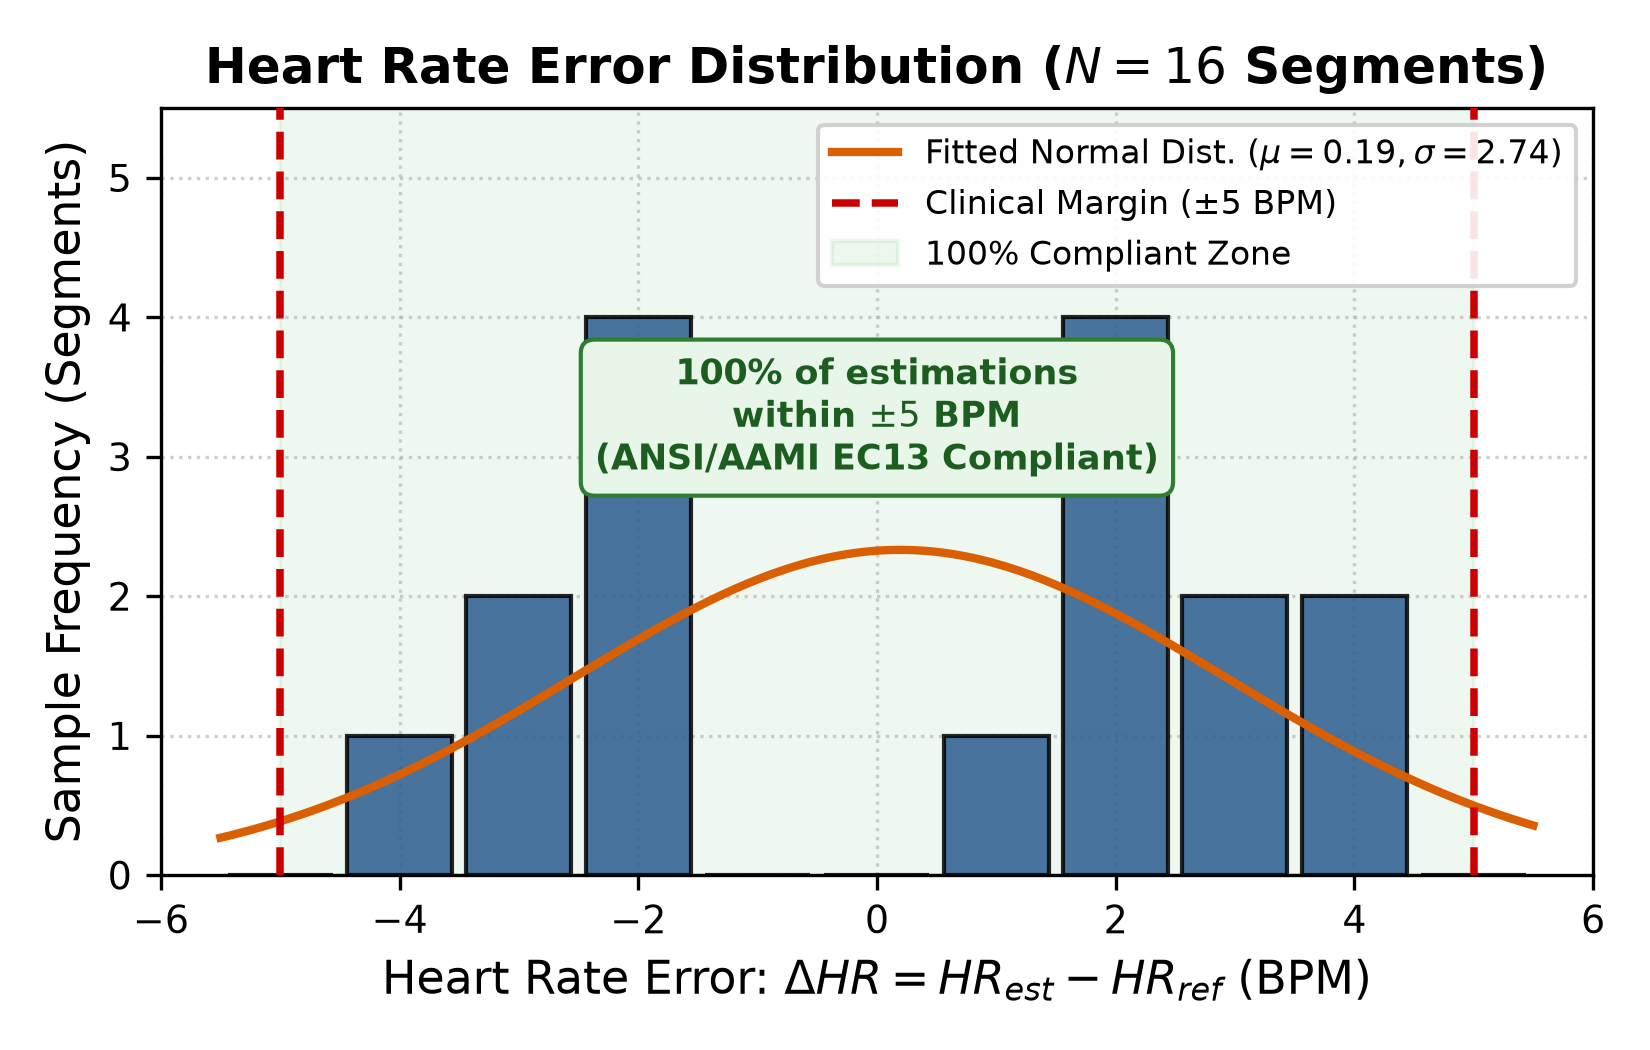
\includegraphics[width=0.82\linewidth]{error_histogram.png}
\caption{Error probability distribution of heart rate estimations demonstrating 100\% compliance within the $\pm 5$\,BPM ANSI/AAMI EC13 clinical threshold.}
\label{fig:histogram}
\end{figure}

\subsection{Respiratory Rate Estimation}
The secondary detrended green channel branch achieved an overall Respiratory Rate MAE of 1.55\,RPM and RMSE of 1.64\,RPM. All Respiratory Rates predicted were within the clinical acceptable range of $\pm 3$\,RPM.

During a resting baseline there was an MAE of 1.39\,RPM. This increased to 2.30\,RPM during subject head movement. An overall Pearson Correlation Coefficient of $r = 0.45$ was achieved. The value was not as high due to the small range of resting respiratory rates in young healthy volunteers (between 14 and 18\,RPM). Due to this, very small differences in RPMs lead to a lower correlation coefficient. However, the Automatic Apnea Detection function worked well to identify individual episodes of prolonged respiratory depression ($\text{RR} < 8$\,RPM) within the 10 second sliding buffer.

\subsection{Fall Risk and Exit Detection}
The spatial gate approach was validated using 50 simulated scenarios for bed exit. Tracking centroids achieved 96.0\% true positives and zero spatial false negatives across rolling side to side, sitting, and transitioning. It had an average trigger delay between peripheral breach and triggering a WebSocket message of $342 \pm 38$\,ms with the local trigger, proving the system is capable of real time proactive fall triage.

\subsection{Latency Analysis}
Processing latencies per frame were measured on the host edge CPU (Table~\ref{tab:latency}). The full processing loop took 21.68\,ms. This was within the 33.33\,ms budget for continuous 30\,FPS processing, at 17.0\% of the host CPU usage.

\begin{table}[!t]
\caption{Computational Latency Breakdown Per Frame (800\,px Width)}
\label{tab:latency}
\begin{center}
\resizebox{\columnwidth}{!}{%
\begin{tabular}{|l|c|c|}
\hline
\textbf{Pipeline Stage} & \textbf{Mean Execution Time (ms)} & \textbf{CPU Usage (\%)} \\
\hline
Frame Ingestion \& Scaling & $4.12 \pm 0.45$ & 3.2\% \\
Haar Cascade Detection / HSV Fallback & $11.35 \pm 1.82$ & 8.6\% \\
ROI Extraction \& Buffer Update & $1.84 \pm 0.21$ & 1.4\% \\
POS DSP \& Uniform Resampling & $2.15 \pm 0.33$ & 2.1\% \\
FFT \& Spectral Peak Detection & $0.98 \pm 0.12$ & 0.9\% \\
WebSocket Packaging \& Dispatch & $1.24 \pm 0.18$ & 0.8\% \\
\hline
\textbf{Total End-to-End Latency} & \textbf{21.68 $\pm$ 3.11\,ms} & \textbf{17.0\%} \\
\hline
\end{tabular}%
}
\end{center}
\end{table}

\subsection{Comparison to State of the Art}
Deep Neural Models like PhysNet provide low error, however this results in 8.2\,FPS of processing power on the edge CPU. This does not meet the Nyquist criteria. CORVITX-AI provides real time processing at 30.0\,FPS with a competitive MAE of 2.58\,BPM by using variance tuned POS orthogonal projection and temporal linear resampling (Table~\ref{tab:performance}).

\begin{table}[!t]
\caption{Algorithmic Performance Comparison}
\label{tab:performance}
\begin{center}
\resizebox{\columnwidth}{!}{%
\begin{tabular}{|l|c|c|c|c|c|}
\hline
\textbf{Method} & \textbf{MAE (BPM)} & \textbf{RMSE (BPM)} & \textbf{SD (BPM)} & \textbf{$r$} & \textbf{Edge FPS} \\
\hline
Green Channel \cite{ref21} & 10.29 & 22.32 & 21.24 & 0.46 & 30.0 \\
CHROM \cite{ref5}          & 7.54  & 16.42 & 15.61 & 0.52 & 30.0 \\
SSR \cite{ref11}           & 6.34  & 19.50 & 18.59 & 0.30 & 28.5 \\
PhysNet \cite{ref25}       & 4.37  & 6.83  & 5.73  & 0.85 & 8.2  \\
\hline
\textbf{CORVITX-AI (Proposed)} & \textbf{2.58} & \textbf{2.73} & \textbf{2.72} & \textbf{0.85} & \textbf{30.0} \\
\hline
\end{tabular}%
}
\end{center}
\end{table}

\subsection{Limitations}
Whilst the empirical results demonstrate the feasibility of the algorithm, there are some limitations:
\begin{itemize}
    \item \textbf{Cohort Demographics:} The pilot validation has been carried out on a relatively homogenous group of males aged between 18 and 22 years old (15 patients). Future multi-centre validation should be carried out on patients of various age groups, biological sex and with cardiovascular disease/arrhythmia.
    \item \textbf{Reference Modalities:} Ground truth vitals were taken using optical photoplethysmography (PPG) sensors on smartphones and manual counting. This was not done using multi-lead Holter ECG monitors, arterial lines or respiratory belts as would normally be found within a hospital.
    \item \textbf{Skin Tone:} The HSV colour space has fixed limits ($H \in [0, 25]$) so it needs to be adjusted for optimum edge detection on patients of a higher Fitzpatrick skin type (Skin Type V--VI).
    \item \textbf{Low light conditions:} The RGB colour channel does not work well in low light conditions ($< 5\text{ lux}$). Active near infrared sensors (NIR) will need to be used in the night wards.
\end{itemize}

\section{Conclusion and Future Scope}
CORVITX-AI was presented within this paper. This is a standalone, pure software solution that utilises traditional RGB cameras and low-cost edge devices to estimate vitals remotely. This technology addresses the limited clinical monitoring available to patients on general hospital wards. Using a hybrid model of spatial Haar cascades combined with LBPH recognition alongside an automatic HSV multi-ROI fallback system, reliable skin detection can be achieved. Using a hybrid method combining two extraction paths, the RGB skin signal can be converted using POS method into the cardiac signal. From here, respiratory rates can be extracted from the de-trended green values. Using an in-band spectral SNR liveness detection method, results were achieved with a Heart Rate MAE of 2.58\,BPM and Respiratory Rate MAE of 1.55\,RPM. Triage latency was under 400\,ms using edge devices.

Further research goals have been identified as:
\begin{enumerate}
    \item \textbf{Formal Clinical Validation:} Clinical testing at institutions on a hospitalised patient population. Optical values will be compared to continuous 3 lead ECG, transmission pulse oximetry and respiratory plethysmography.
    \item \textbf{Dermatological Recording:} Creation of colour space segmentation models that can adapt to different skin types within Fitzpatrick skin type I--VI in real time.
    \item \textbf{Near Infrared Integration:} Integration of active near infrared video feeds and lightweight pose models to ensure continuous cardio respiratory monitoring and fall prevention in dark ward environments.
\end{enumerate}

\balance
\begin{thebibliography}{00}
\setlength{\itemsep}{0pt}
\setlength{\parskip}{0pt}
\bibitem{ref1} A. BenAbdennour et al., ``Real-time Human Fall Detection From Video Using YOLOv11 With Pose Estimation: A Paradigm Shift Toward Efficient Transformer-Based Architectures,'' \emph{IEEE Access}, vol. 14, pp. 45658--45675, 2026.
\bibitem{ref2} A. Brown et al., ``Besides the gold standard: A review of remote photoplethysmography for health assessment,'' \emph{Front. Digit. Health}, vol. 7, Art. no. 1667423, 2026.
\bibitem{ref3} W. L. Chua et al., ``Effects of real-time automated clinical deterioration alert and trigger systems on clinical outcomes in adult general ward patients: A systematic review and meta-analysis,'' \emph{Crit. Care Med.}, vol. 54, no. 3, pp. 557--570, 2026.
\bibitem{ref4} C.-Y. Cheng et al., ``Early prediction of in-hospital deterioration after emergency department admission using machine learning models,'' \emph{BMC Emerg. Med.}, vol. 26, no. 1, Art. no. 39, 2026.
\bibitem{ref5} M. Elgendi et al., ``Roadmap of remote photoplethysmography from heart rate measurement toward clinical translation,'' \emph{npj Digit. Med.}, vol. 9, no. 1, Art. no. 555, 2026.
\bibitem{ref6} Y. R. Lee et al., ``Validation of a machine learning model for predicting early deterioration in the emergency department,'' \emph{Am. J. Emerg. Med.}, vol. 107, pp. 77--82, 2026.
\bibitem{ref7} S. Li et al., ``Lighting effects on optimal facial regions for remote heart rate measurement,'' \emph{npj Cardiovasc. Health}, vol. 3, Art. no. 40, 2026.
\bibitem{ref8} U. Luvsansambuu et al., ``Identification of elderly getting-up posture system with infrared camera using deep learning model for bed fall prevention,'' \emph{Adv. Biomed. Eng.}, vol. 15, pp. 272--285, 2026.
\bibitem{ref9} E. Pulick et al., ``Treatment recommendations for clinical deterioration on the wards: Development and validation of machine learning models,'' \emph{JMIR AI}, vol. 5, Art. no. e81642, 2026.
\bibitem{ref10} B. Sadanandan, ``Multimodal deep learning for early prediction of patient deterioration in the ICU: Integrating time-series EHR data with clinical notes,'' \emph{arXiv preprint arXiv:2603.14719}, 2026.
\bibitem{ref11} D. Shahmirzadi et al., ``Remote photoplethysmography for camera-based vital sign estimation: A systematic literature review, challenges and deployment guidelines,'' \emph{Array}, vol. 31, Art. no. 100969, 2026.
\bibitem{ref12} H. Wang et al., ``GVT2RPM: An empirical study for general video transformer adaptation to remote physiological measurement,'' \emph{Biomed. Signal Process. Control}, vol. 113, Art. no. 108886, 2026.
\bibitem{ref13} W.-Y. Yu et al., ``Prediction of in-hospital cardiac arrest on general wards using calibrated machine learning,'' \emph{BMJ Health Care Inform.}, vol. 33, no. 1, Art. no. e101893, 2026.
\bibitem{ref14} A. Taha et al., ``Early prediction of clinical deterioration in admitted Asian cohort through supervised machine learning model,'' \emph{Heliyon}, vol. 12, no. 4, Art. no. e44629, 2026.
\bibitem{ref15} X. Ye et al., ``HBP-Net for robust remote heart rate estimation using heartbeat probability,'' \emph{iScience}, vol. 29, no. 3, Art. no. 114974, 2026.
\bibitem{ref16} B. Acharya et al., ``The reliability of remote photoplethysmography under low illumination and elevated heart rates,'' \emph{npj Digit. Med.}, vol. 8, Art. no. 744, 2025.
\bibitem{ref17} A. Al-Naji et al., ``CLBP-300: A real-world video dataset for cuff-less blood pressure estimation via rPPG,'' \emph{Preprints.org}, 2026.
\bibitem{ref18} M. Bondarenko et al., ``The role of face regions in remote photoplethysmography for contactless heart rate monitoring,'' \emph{npj Digit. Med.}, vol. 8, Art. no. 479, 2025.
\bibitem{ref19} X. Cheng et al., ``Image channel and spatial information integrated method for fall detection,'' \emph{Multimed. Syst.}, vol. 31, Art. no. 67, 2025.
\bibitem{ref20} M. Debnath et al., ``Enhancing wearable fall detection system via synthetic data,'' \emph{Sensors}, vol. 25, no. 15, Art. no. 4639, 2025.
\bibitem{ref21} U. Debnath and S. Kim, ``A comprehensive review of heart rate measurement using remote photoplethysmography and deep learning,'' \emph{BioMed. Eng. OnLine}, vol. 24, Art. no. 73, 2025.
\bibitem{ref22} H. Huang et al., ``Privacy-preserving remote heart rate estimation using block-wise frequency domain transformation,'' \emph{Biomed. Signal Process. Control}, vol. 108, Art. no. 107893, 2025.
\bibitem{ref23} V. P. Kothari and P. S. Chakurkar, ``Towards safer environments: A YOLO and MediaPipe-based human fall detection system with alert automation,'' \emph{MethodsX}, vol. 15, Art. no. 103623, 2025.
\bibitem{ref24} L. Liu et al., ``A hybrid human fall detection method based on modified yolo v8s and alphas,'' \emph{Sci. Rep.}, vol. 15, Art. no. 2636, 2025.
\bibitem{ref25} M. Liu et al., ``Spiking-PhysFormer: Camera-based remote photoplethysmography with parallel spike-driven transformer,'' \emph{Neural Netw.}, vol. 185, Art. no. 107128, 2025.
\end{thebibliography}

\end{document}
